\chapter{Introduction}

\section{Optical Microscopy}

Optical microscopy is one of the oldest scientific instruments of the sciences, and continues to be an essential tool for researchers, clinicians, and engineers across many disciplines. Different from spectacles, which use a single lens to provide magnification for one or both eyes, microscopes are typically defined as having two or more refractive surfaces to provide magnification between the object of interest and the imaging plane, enabling the user to see things much smaller than the normal optical resolution of the human eye. Credit for the inventor of the compound microscope is generally attributed to Hans and Zacharias Jansen of the Netherlands, although the first published work on microscope design wasn't released until 1665 (Hooke and van Leeuwenhoek) \cite{natureMilestones,hookeMicrographica}. The term "microscope" may refer to any system which magnifies a small object for viewing using the eyes or camera. In this work, our discussion of microscopes will be limited to optical microscopes - those which are designed for use with light within the optical band of the electro-magnetic spectrum ($390nm \leq \lambda \leq 700nm$), which is approximately the electromagnetic spectrum detectable by the human eye.

\subsection{Imaging and Resolution}
Generally speaking, a single lens may be used to form a magnified image of a sample - this is a simple consequence of the imaging condition,

\begin{equation}
\frac{1}{f} = \frac{1}{s_o} + \frac{1}{s_i}
\end{equation}

Which relates the distance of an optical element to a object under observation $s_o$ to the distance of a conjugate image $s_i$, which may be magnified by a factor $M = \frac{-s_i}{s_o}$ based on the relative distances of each quantity. The variable $f$ corresponds to the focal length of the element, which may also be an effective focal length from the combination of several refractive elements. While this optical system will magnify an object if $M > 1$, it is practically limited to smaller magnifications since there is normally a practical upper limit on $s_o$ (set by working distance) and a lower limit on the distance of the image from the lens $s_i$ (due to eyepiece design).

The compound microscope takes advantage of multiple refractive elements to form an image. Typically, the exact number and design of these components is abstracted to the end-user, and can be defined by a relatively low number of descriptive quantities despite the complex internal lens design of a modern microscope objective. Magnification and Numerical Aperture (NA) are the most important of these physical quantities; the magnification of an objective sets the field of view which is relayed by the optic, while the numerical aperture sets a minimum bound on the resolution of the optic, often called the diffraction limit. Numerical Aperture is defined by the formula $NA=n\sin (\theta)$, where $n$ is the refractive index of the medium, and $\theta$ is the maximum half-angle at which light may pass through the objective relative to the radial (optical) axis. The angular dependance of Numerical Aperture is completely described by interference effects which arise from the wave-optics model of light propagation. As multiple off-axis sources of the same wavelength converge to a point, the wavefronts of these sources will cause constructive and destructive interference; The size of the smallest area of constructive interference is proportional to both the wavelength of the illumination and the angular separation between the two beams. Practically, the size of this spot defines the resolution of the optical system. By the Rayleigh criteria, the resolution of an optical system is set by:

\begin{equation}
\Delta x_{min}  = \frac{1.22 \lambda}{(NA_{objective} + NA_{illumination})}
\end{equation}

This Rayleigh criterion defines the minimum separation between two points which can be detected by a system with a circular aperture, and is defined by the distance between the center if the point spread function (PSF) and it's first null. This formulation combines both detection side NA ($NA_{objective}$) and illumination side NA ($NA_{illumination}$). The ratio between these NA, typically denoted as $\sigma = NA_{objective}/NA_{Illumination}$, is commonly known as the coherence factor. As $\sigma \longrightarrow 0 $, the illumination becomes spatially coherent, meaning the phase of the illumination wavefront at a given point on the sample can be perfectly defined by all other points on the sample. This definition assumes that the light source is composed of spatially distributed statistically uncorrelated emitters - normal sources such as halogen and tungsten lamps satisfy this criteria while in k{\"o}hler geometry. As sigma increases, the minimum resolvable feature size decreases, leading to images of higher quality, subject to aliasing affects. However, increasing $\sigma$ beyond 1 does not provide further resolution improvement due to the ballistic light (DC term) is not collected by the objective. This is the working principle of dark-field microscopy. Achieving resolution improvements beyond $2\times NA_{objective}$  require computational imaging techniques such as structured illumination \cite{gustafsson2000surpassing} or Fourier ptychography\cite{Zheng2013}.

\subsection{Fourier Optics Description}
The sub-field of Fourier optics provides a theoretical bridge between conventional optics and signal processing. In modern microscopes, digital cameras allow the detection of the Intensity of an optical field using a grid of photodetectors, which readily enables the use of digital signal processing techniques on images formed by a microscope. Fourier optics is especially useful for an optical system configured as a 4$f$ system:

\begin{figure}[tbh]
\centering
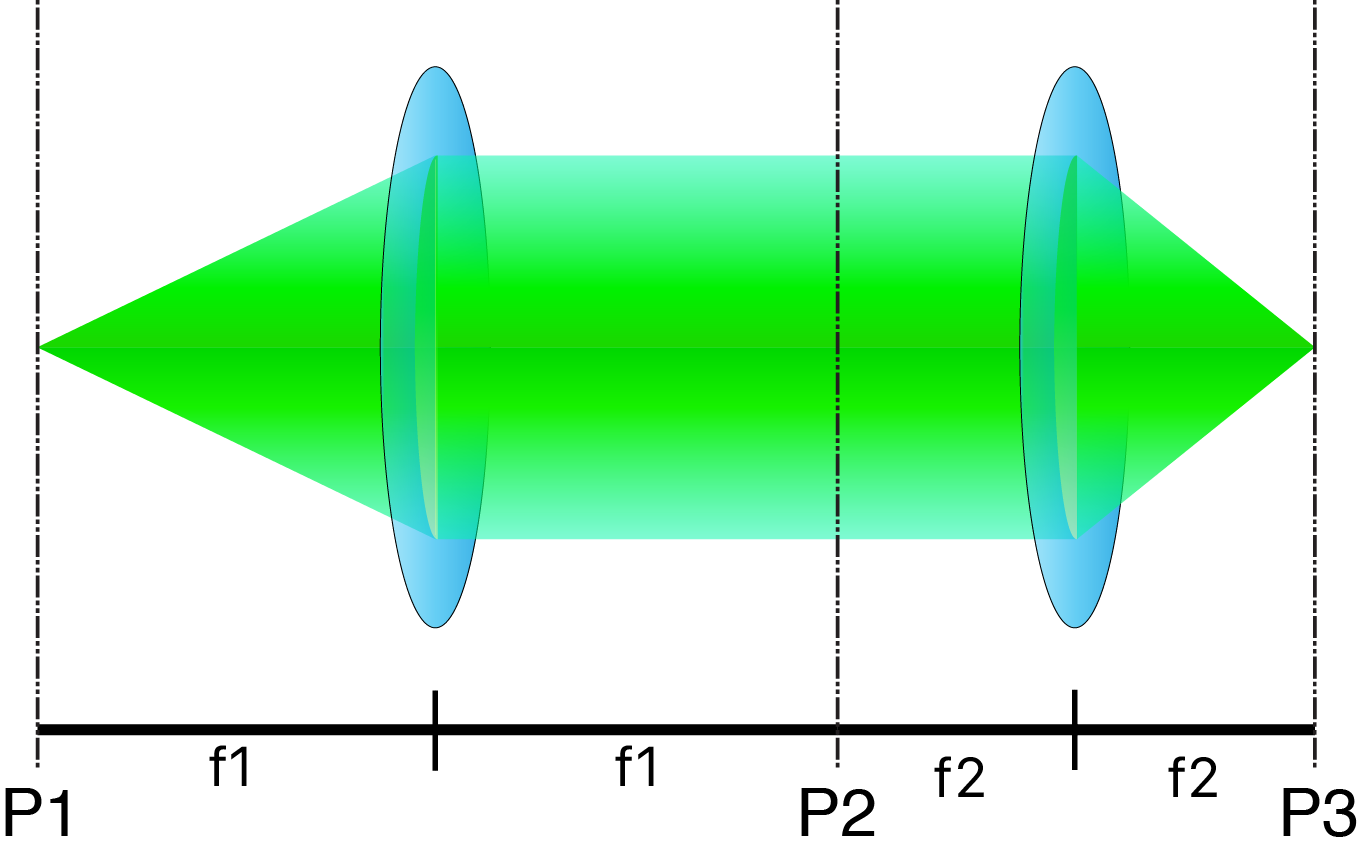
\includegraphics[width=0.4\textwidth]{intro-4f.png}
\caption{\label{fig:4f} Schematic of a 4$f$ optical system}
\end{figure}

In this optical configuration, the lenses in this system operate as forward and inverse Fourier Transform operators on the optical field at P1 up to a given range of support set by the NA of the lens. The Fourier Transform of P1 exists at position P2, which is often occupied by an aperture stop to limit the NA of the objective. This aperture stop prevents stray or highly abberated rays from entering the imaging plane and prevents aliasing, which is a phenomena caused by sampling a signal at a frequency which is below a the so-called Nyquist frequency, defined by the bandwidth of the measurement. In an optical system, this frequency is set by the pixel separation and system magnification relative to the imaging NA of the system.

\section{Phase Imaging}
Visible light, like any electromagnetic (EM) radiation, is a propagating wave, and thus has both amplitude and phase. As a single coherent mode of light interacts with a general object it can be absorbed (reduced in amplitude), or reflected, refracted, or diffracted (change in phase) based on the material properties and geometry of the object. Measuring this complete electromagnetic field at the sample plane is the primary goal of an imaging system; however, current camera technology can only measure the amplitude modulation of a sample due to a finite integration time of the sensor over many periods of the arriving optical wavefront. Mathematically, this process is described as taking the magnitude of the complex field $I =|E|^2 =|Ae^{i\phi}|^2 = A^2$ where $A$ is the amplitude of a wave and $\phi$ is the phase of the wavefront in this phasor notation. Phase is related to the mechanical geometry of the cell by the relationship $\phi = \frac{2\pi}{\lambda} n d$, where $\lambda$ is the system wavelength, $n$ is the refractive index change, and $d$ is the thickness of the object.

This loss of phase information is particularly problematic for imaging aqueous samples such as cells. To counter this, biologists often apply chemical stains to add absorption contrast artificially, but this process is cumbersome and can modify the micro-environment in significant ways. Early phase imaging methods such as Differential Interference Contrast (DIC)\cite{smithDIC} and Zernike Phase Contrast (PhC) \cite{zernike1955discovered} were developed to solve this issue using interferometric tricks to mix phase and amplitude into the measurements, providing contrast for transparent specimens. These methods have since become widely adopted due to these advantages.

\section{Computational Imaging}
Computational Imaging is a recent concept which has emerged due to increasing availability of computing power and digital sensing hardware. In a Fourier optics model, an optical system can be approximated as a linear system, enabling the application of a large number of algorithms such as least squares, gradient descent, and nonlinear optimization techniques. Computational Imaging takes advantage of this mathematical description to move part of the image formation process from hardware to software. This paradigm shift enables image formation processes that were previously infeasible for conventional optical imaging, allowing an optical system designer to take advantage of the strengths of both hardware and software during each step of the image formation process.  An early example of computational imaging was the application of a cubic phase plate at the microscope pupil, which provides drastically increased depth of field but produces a highly distorted image. Since these distortions are known, however, the original image with extended depth of field can be deconvolved using knowledge of the system's point spread function (PSF)\cite{Dowski:95}. This general framework of this deconvolution problem can be represented as an inverse problem of the form:

\begin{equation}
\begin{aligned}
& \hat{x} = \underset{x}{\text{argmin}}
& & ||Ax-I ||_2^2
\end{aligned}
\end{equation}

Where $x$ represents the variable of interest (generally the object), $A$ is the forward system matrix operator, and $I$ is the measured intensity. This is the general formulation of a linear inverse problem, and is solved in various ways depending on the structure of $A$.

In the following chapters I will describe several applications of computational imaging in optical microscopy. Chapter 2 will cover a single-shot quantitative phase imaging method which uses partially coherent color illumination to recover the complete optical field of an object from a single measurement. Chapter 3 describes an extension of this method which allows for the deblurring of an object's complete optical field as it moves across the field of view during an exposure, assuming prior knowledge of the blurring process. Chapter 4 describes Computational CellScope, a prototype device which uses a programmable domed LED illumination to perform quantitative phase imaging, digital refocusing, and multi-contrast imaging in a portable package using a smartphone for both acquisition and processing. Chapter 5 concludes this thesis and provides possible extensions of the work presented in the previous chapters.
